% Created by tikzDevice version 0.9 on 2015-12-16 19:00:50
% !TEX encoding = UTF-8 Unicode
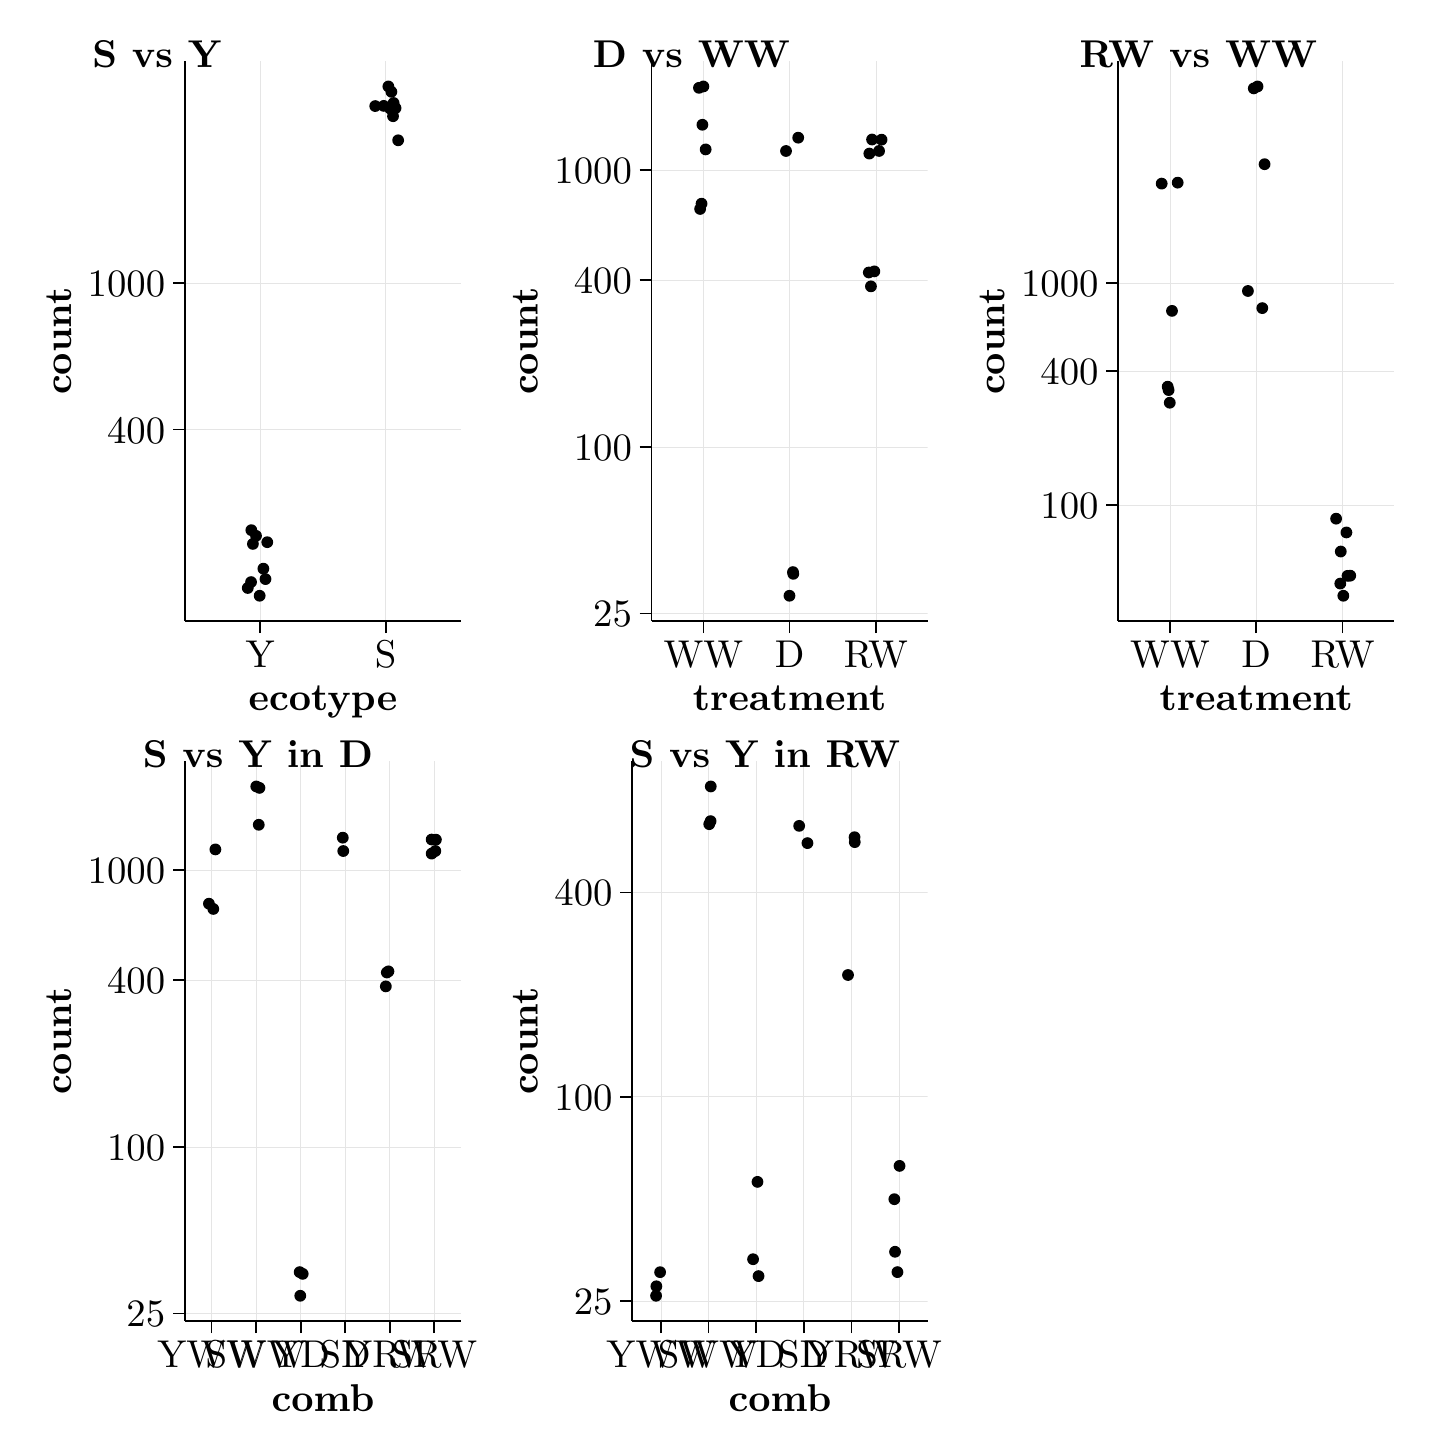
\begin{tikzpicture}[x=1pt,y=1pt]
\definecolor{fillColor}{RGB}{255,255,255}
\path[use as bounding box,fill=fillColor,fill opacity=0.00] (0,0) rectangle (505.89,505.89);
\begin{scope}
\path[clip] (  0.00,  0.00) rectangle (505.89,505.89);

\path[] (  0.00,  0.00) rectangle (505.89,505.89);
\end{scope}
\begin{scope}
\path[clip] ( 56.81,291.41) rectangle (156.58,493.85);
\definecolor{drawColor}{gray}{0.90}

\path[draw=drawColor,line width= 0.2pt,line join=round] ( 56.81,360.63) --
	(156.58,360.63);

\path[draw=drawColor,line width= 0.2pt,line join=round] ( 56.81,413.70) --
	(156.58,413.70);

\path[draw=drawColor,line width= 0.2pt,line join=round] ( 84.02,291.41) --
	( 84.02,493.85);

\path[draw=drawColor,line width= 0.2pt,line join=round] (129.37,291.41) --
	(129.37,493.85);
\definecolor{fillColor}{RGB}{0,0,0}

\path[fill=fillColor] (132.23,478.67) circle (  2.13);

\path[fill=fillColor] (132.02,473.89) circle (  2.13);

\path[fill=fillColor] (130.34,484.64) circle (  2.13);

\path[fill=fillColor] (131.43,482.71) circle (  2.13);

\path[fill=fillColor] (128.67,477.62) circle (  2.13);

\path[fill=fillColor] (132.93,476.82) circle (  2.13);

\path[fill=fillColor] (133.87,465.19) circle (  2.13);

\path[fill=fillColor] (125.59,477.56) circle (  2.13);

\path[fill=fillColor] (130.99,476.63) circle (  2.13);

\path[fill=fillColor] ( 86.57,319.96) circle (  2.13);

\path[fill=fillColor] ( 80.72,305.55) circle (  2.13);

\path[fill=fillColor] ( 85.93,306.64) circle (  2.13);

\path[fill=fillColor] ( 82.51,322.27) circle (  2.13);

\path[fill=fillColor] ( 81.39,319.34) circle (  2.13);

\path[fill=fillColor] ( 80.82,324.31) circle (  2.13);

\path[fill=fillColor] ( 85.17,310.40) circle (  2.13);

\path[fill=fillColor] ( 83.83,300.61) circle (  2.13);

\path[fill=fillColor] ( 79.53,303.42) circle (  2.13);
\end{scope}
\begin{scope}
\path[clip] (  0.00,  0.00) rectangle (505.89,505.89);
\definecolor{drawColor}{RGB}{0,0,0}

\path[draw=drawColor,line width= 0.6pt,line join=round] ( 56.81,291.41) --
	( 56.81,493.85);
\end{scope}
\begin{scope}
\path[clip] (  0.00,  0.00) rectangle (505.89,505.89);
\definecolor{drawColor}{RGB}{0,0,0}

\node[text=drawColor,anchor=base east,inner sep=0pt, outer sep=0pt, scale=  1.40] at ( 49.70,355.81) {400};

\node[text=drawColor,anchor=base east,inner sep=0pt, outer sep=0pt, scale=  1.40] at ( 49.70,408.88) {1000};
\end{scope}
\begin{scope}
\path[clip] (  0.00,  0.00) rectangle (505.89,505.89);
\definecolor{drawColor}{RGB}{0,0,0}

\path[draw=drawColor,line width= 0.6pt,line join=round] ( 52.54,360.63) --
	( 56.81,360.63);

\path[draw=drawColor,line width= 0.6pt,line join=round] ( 52.54,413.70) --
	( 56.81,413.70);
\end{scope}
\begin{scope}
\path[clip] (  0.00,  0.00) rectangle (505.89,505.89);
\definecolor{drawColor}{RGB}{0,0,0}

\path[draw=drawColor,line width= 0.6pt,line join=round] ( 56.81,291.41) --
	(156.58,291.41);
\end{scope}
\begin{scope}
\path[clip] (  0.00,  0.00) rectangle (505.89,505.89);
\definecolor{drawColor}{RGB}{0,0,0}

\path[draw=drawColor,line width= 0.6pt,line join=round] ( 84.02,287.14) --
	( 84.02,291.41);

\path[draw=drawColor,line width= 0.6pt,line join=round] (129.37,287.14) --
	(129.37,291.41);
\end{scope}
\begin{scope}
\path[clip] (  0.00,  0.00) rectangle (505.89,505.89);
\definecolor{drawColor}{RGB}{0,0,0}

\node[text=drawColor,anchor=base,inner sep=0pt, outer sep=0pt, scale=  1.40] at ( 84.02,274.65) {Y};

\node[text=drawColor,anchor=base,inner sep=0pt, outer sep=0pt, scale=  1.40] at (129.37,274.65) {S};
\end{scope}
\begin{scope}
\path[clip] (  0.00,  0.00) rectangle (505.89,505.89);
\definecolor{drawColor}{RGB}{0,0,0}

\node[text=drawColor,anchor=base,inner sep=0pt, outer sep=0pt, scale=  1.40] at (106.70,258.97) {\bfseries ecotype};
\end{scope}
\begin{scope}
\path[clip] (  0.00,  0.00) rectangle (505.89,505.89);
\definecolor{drawColor}{RGB}{0,0,0}

\node[text=drawColor,rotate= 90.00,anchor=base,inner sep=0pt, outer sep=0pt, scale=  1.40] at ( 15.68,392.63) {\bfseries count};
\end{scope}
\begin{scope}
\path[clip] (  0.00,  0.00) rectangle (505.89,505.89);
\definecolor{drawColor}{RGB}{0,0,0}

\node[text=drawColor,anchor=base west,inner sep=0pt, outer sep=0pt, scale=  1.40] at ( 23.34,491.40) {\bfseries S vs Y};
\end{scope}
\begin{scope}
\path[clip] (225.44,291.41) rectangle (325.21,493.85);
\definecolor{drawColor}{gray}{0.90}

\path[draw=drawColor,line width= 0.2pt,line join=round] (225.44,294.15) --
	(325.21,294.15);

\path[draw=drawColor,line width= 0.2pt,line join=round] (225.44,354.38) --
	(325.21,354.38);

\path[draw=drawColor,line width= 0.2pt,line join=round] (225.44,414.60) --
	(325.21,414.60);

\path[draw=drawColor,line width= 0.2pt,line join=round] (225.44,454.41) --
	(325.21,454.41);

\path[draw=drawColor,line width= 0.2pt,line join=round] (244.15,291.41) --
	(244.15,493.85);

\path[draw=drawColor,line width= 0.2pt,line join=round] (275.33,291.41) --
	(275.33,493.85);

\path[draw=drawColor,line width= 0.2pt,line join=round] (306.51,291.41) --
	(306.51,493.85);
\definecolor{fillColor}{RGB}{0,0,0}

\path[fill=fillColor] (274.03,461.32) circle (  2.13);

\path[fill=fillColor] (278.43,466.13) circle (  2.13);

\path[fill=fillColor] (307.65,461.33) circle (  2.13);

\path[fill=fillColor] (304.13,460.39) circle (  2.13);

\path[fill=fillColor] (308.55,465.41) circle (  2.13);

\path[fill=fillColor] (305.11,465.47) circle (  2.13);

\path[fill=fillColor] (243.81,470.80) circle (  2.13);

\path[fill=fillColor] (242.57,484.14) circle (  2.13);

\path[fill=fillColor] (244.16,484.64) circle (  2.13);

\path[fill=fillColor] (275.27,300.61) circle (  2.13);

\path[fill=fillColor] (276.54,309.16) circle (  2.13);

\path[fill=fillColor] (276.66,308.53) circle (  2.13);

\path[fill=fillColor] (304.71,412.41) circle (  2.13);

\path[fill=fillColor] (305.94,417.82) circle (  2.13);

\path[fill=fillColor] (303.94,417.42) circle (  2.13);

\path[fill=fillColor] (244.99,461.89) circle (  2.13);

\path[fill=fillColor] (243.50,442.28) circle (  2.13);

\path[fill=fillColor] (242.99,440.38) circle (  2.13);
\end{scope}
\begin{scope}
\path[clip] (  0.00,  0.00) rectangle (505.89,505.89);
\definecolor{drawColor}{RGB}{0,0,0}

\path[draw=drawColor,line width= 0.6pt,line join=round] (225.44,291.41) --
	(225.44,493.85);
\end{scope}
\begin{scope}
\path[clip] (  0.00,  0.00) rectangle (505.89,505.89);
\definecolor{drawColor}{RGB}{0,0,0}

\node[text=drawColor,anchor=base east,inner sep=0pt, outer sep=0pt, scale=  1.40] at (218.33,289.33) {25};

\node[text=drawColor,anchor=base east,inner sep=0pt, outer sep=0pt, scale=  1.40] at (218.33,349.56) {100};

\node[text=drawColor,anchor=base east,inner sep=0pt, outer sep=0pt, scale=  1.40] at (218.33,409.78) {400};

\node[text=drawColor,anchor=base east,inner sep=0pt, outer sep=0pt, scale=  1.40] at (218.33,449.59) {1000};
\end{scope}
\begin{scope}
\path[clip] (  0.00,  0.00) rectangle (505.89,505.89);
\definecolor{drawColor}{RGB}{0,0,0}

\path[draw=drawColor,line width= 0.6pt,line join=round] (221.17,294.15) --
	(225.44,294.15);

\path[draw=drawColor,line width= 0.6pt,line join=round] (221.17,354.38) --
	(225.44,354.38);

\path[draw=drawColor,line width= 0.6pt,line join=round] (221.17,414.60) --
	(225.44,414.60);

\path[draw=drawColor,line width= 0.6pt,line join=round] (221.17,454.41) --
	(225.44,454.41);
\end{scope}
\begin{scope}
\path[clip] (  0.00,  0.00) rectangle (505.89,505.89);
\definecolor{drawColor}{RGB}{0,0,0}

\path[draw=drawColor,line width= 0.6pt,line join=round] (225.44,291.41) --
	(325.21,291.41);
\end{scope}
\begin{scope}
\path[clip] (  0.00,  0.00) rectangle (505.89,505.89);
\definecolor{drawColor}{RGB}{0,0,0}

\path[draw=drawColor,line width= 0.6pt,line join=round] (244.15,287.14) --
	(244.15,291.41);

\path[draw=drawColor,line width= 0.6pt,line join=round] (275.33,287.14) --
	(275.33,291.41);

\path[draw=drawColor,line width= 0.6pt,line join=round] (306.51,287.14) --
	(306.51,291.41);
\end{scope}
\begin{scope}
\path[clip] (  0.00,  0.00) rectangle (505.89,505.89);
\definecolor{drawColor}{RGB}{0,0,0}

\node[text=drawColor,anchor=base,inner sep=0pt, outer sep=0pt, scale=  1.40] at (244.15,274.65) {WW};

\node[text=drawColor,anchor=base,inner sep=0pt, outer sep=0pt, scale=  1.40] at (275.33,274.65) {D};

\node[text=drawColor,anchor=base,inner sep=0pt, outer sep=0pt, scale=  1.40] at (306.51,274.65) {RW};
\end{scope}
\begin{scope}
\path[clip] (  0.00,  0.00) rectangle (505.89,505.89);
\definecolor{drawColor}{RGB}{0,0,0}

\node[text=drawColor,anchor=base,inner sep=0pt, outer sep=0pt, scale=  1.40] at (275.33,258.97) {\bfseries treatment};
\end{scope}
\begin{scope}
\path[clip] (  0.00,  0.00) rectangle (505.89,505.89);
\definecolor{drawColor}{RGB}{0,0,0}

\node[text=drawColor,rotate= 90.00,anchor=base,inner sep=0pt, outer sep=0pt, scale=  1.40] at (184.31,392.63) {\bfseries count};
\end{scope}
\begin{scope}
\path[clip] (  0.00,  0.00) rectangle (505.89,505.89);
\definecolor{drawColor}{RGB}{0,0,0}

\node[text=drawColor,anchor=base west,inner sep=0pt, outer sep=0pt, scale=  1.40] at (204.23,491.40) {\bfseries D vs WW};
\end{scope}
\begin{scope}
\path[clip] (394.07,291.41) rectangle (493.85,493.85);
\definecolor{drawColor}{gray}{0.90}

\path[draw=drawColor,line width= 0.2pt,line join=round] (394.07,333.38) --
	(493.85,333.38);

\path[draw=drawColor,line width= 0.2pt,line join=round] (394.07,381.71) --
	(493.85,381.71);

\path[draw=drawColor,line width= 0.2pt,line join=round] (394.07,413.65) --
	(493.85,413.65);

\path[draw=drawColor,line width= 0.2pt,line join=round] (412.78,291.41) --
	(412.78,493.85);

\path[draw=drawColor,line width= 0.2pt,line join=round] (443.96,291.41) --
	(443.96,493.85);

\path[draw=drawColor,line width= 0.2pt,line join=round] (475.14,291.41) --
	(475.14,493.85);
\definecolor{fillColor}{RGB}{0,0,0}

\path[fill=fillColor] (440.93,410.74) circle (  2.13);

\path[fill=fillColor] (446.12,404.55) circle (  2.13);

\path[fill=fillColor] (472.80,328.46) circle (  2.13);

\path[fill=fillColor] (476.52,323.48) circle (  2.13);

\path[fill=fillColor] (475.40,300.61) circle (  2.13);

\path[fill=fillColor] (477.91,307.87) circle (  2.13);

\path[fill=fillColor] (412.69,370.36) circle (  2.13);

\path[fill=fillColor] (411.94,376.15) circle (  2.13);

\path[fill=fillColor] (412.27,374.93) circle (  2.13);

\path[fill=fillColor] (446.95,456.55) circle (  2.13);

\path[fill=fillColor] (443.05,483.94) circle (  2.13);

\path[fill=fillColor] (444.40,484.64) circle (  2.13);

\path[fill=fillColor] (474.31,305.01) circle (  2.13);

\path[fill=fillColor] (474.48,316.59) circle (  2.13);

\path[fill=fillColor] (476.92,307.80) circle (  2.13);

\path[fill=fillColor] (413.50,403.55) circle (  2.13);

\path[fill=fillColor] (415.55,449.88) circle (  2.13);

\path[fill=fillColor] (409.77,449.54) circle (  2.13);
\end{scope}
\begin{scope}
\path[clip] (  0.00,  0.00) rectangle (505.89,505.89);
\definecolor{drawColor}{RGB}{0,0,0}

\path[draw=drawColor,line width= 0.6pt,line join=round] (394.07,291.41) --
	(394.07,493.85);
\end{scope}
\begin{scope}
\path[clip] (  0.00,  0.00) rectangle (505.89,505.89);
\definecolor{drawColor}{RGB}{0,0,0}

\node[text=drawColor,anchor=base east,inner sep=0pt, outer sep=0pt, scale=  1.40] at (386.96,328.56) {100};

\node[text=drawColor,anchor=base east,inner sep=0pt, outer sep=0pt, scale=  1.40] at (386.96,376.89) {400};

\node[text=drawColor,anchor=base east,inner sep=0pt, outer sep=0pt, scale=  1.40] at (386.96,408.83) {1000};
\end{scope}
\begin{scope}
\path[clip] (  0.00,  0.00) rectangle (505.89,505.89);
\definecolor{drawColor}{RGB}{0,0,0}

\path[draw=drawColor,line width= 0.6pt,line join=round] (389.80,333.38) --
	(394.07,333.38);

\path[draw=drawColor,line width= 0.6pt,line join=round] (389.80,381.71) --
	(394.07,381.71);

\path[draw=drawColor,line width= 0.6pt,line join=round] (389.80,413.65) --
	(394.07,413.65);
\end{scope}
\begin{scope}
\path[clip] (  0.00,  0.00) rectangle (505.89,505.89);
\definecolor{drawColor}{RGB}{0,0,0}

\path[draw=drawColor,line width= 0.6pt,line join=round] (394.07,291.41) --
	(493.85,291.41);
\end{scope}
\begin{scope}
\path[clip] (  0.00,  0.00) rectangle (505.89,505.89);
\definecolor{drawColor}{RGB}{0,0,0}

\path[draw=drawColor,line width= 0.6pt,line join=round] (412.78,287.14) --
	(412.78,291.41);

\path[draw=drawColor,line width= 0.6pt,line join=round] (443.96,287.14) --
	(443.96,291.41);

\path[draw=drawColor,line width= 0.6pt,line join=round] (475.14,287.14) --
	(475.14,291.41);
\end{scope}
\begin{scope}
\path[clip] (  0.00,  0.00) rectangle (505.89,505.89);
\definecolor{drawColor}{RGB}{0,0,0}

\node[text=drawColor,anchor=base,inner sep=0pt, outer sep=0pt, scale=  1.40] at (412.78,274.65) {WW};

\node[text=drawColor,anchor=base,inner sep=0pt, outer sep=0pt, scale=  1.40] at (443.96,274.65) {D};

\node[text=drawColor,anchor=base,inner sep=0pt, outer sep=0pt, scale=  1.40] at (475.14,274.65) {RW};
\end{scope}
\begin{scope}
\path[clip] (  0.00,  0.00) rectangle (505.89,505.89);
\definecolor{drawColor}{RGB}{0,0,0}

\node[text=drawColor,anchor=base,inner sep=0pt, outer sep=0pt, scale=  1.40] at (443.96,258.97) {\bfseries treatment};
\end{scope}
\begin{scope}
\path[clip] (  0.00,  0.00) rectangle (505.89,505.89);
\definecolor{drawColor}{RGB}{0,0,0}

\node[text=drawColor,rotate= 90.00,anchor=base,inner sep=0pt, outer sep=0pt, scale=  1.40] at (352.94,392.63) {\bfseries count};
\end{scope}
\begin{scope}
\path[clip] (  0.00,  0.00) rectangle (505.89,505.89);
\definecolor{drawColor}{RGB}{0,0,0}

\node[text=drawColor,anchor=base west,inner sep=0pt, outer sep=0pt, scale=  1.40] at (380.15,491.40) {\bfseries RW vs WW};
\end{scope}
\begin{scope}
\path[clip] ( 56.81, 38.46) rectangle (156.58,240.90);
\definecolor{drawColor}{gray}{0.90}

\path[draw=drawColor,line width= 0.2pt,line join=round] ( 56.81, 41.21) --
	(156.58, 41.21);

\path[draw=drawColor,line width= 0.2pt,line join=round] ( 56.81,101.43) --
	(156.58,101.43);

\path[draw=drawColor,line width= 0.2pt,line join=round] ( 56.81,161.66) --
	(156.58,161.66);

\path[draw=drawColor,line width= 0.2pt,line join=round] ( 56.81,201.47) --
	(156.58,201.47);

\path[draw=drawColor,line width= 0.2pt,line join=round] ( 66.47, 38.46) --
	( 66.47,240.90);

\path[draw=drawColor,line width= 0.2pt,line join=round] ( 82.56, 38.46) --
	( 82.56,240.90);

\path[draw=drawColor,line width= 0.2pt,line join=round] ( 98.65, 38.46) --
	( 98.65,240.90);

\path[draw=drawColor,line width= 0.2pt,line join=round] (114.75, 38.46) --
	(114.75,240.90);

\path[draw=drawColor,line width= 0.2pt,line join=round] (130.84, 38.46) --
	(130.84,240.90);

\path[draw=drawColor,line width= 0.2pt,line join=round] (146.93, 38.46) --
	(146.93,240.90);
\definecolor{fillColor}{RGB}{0,0,0}

\path[fill=fillColor] (114.04,208.37) circle (  2.13);

\path[fill=fillColor] (113.86,213.19) circle (  2.13);

\path[fill=fillColor] (147.31,208.38) circle (  2.13);

\path[fill=fillColor] (145.98,207.44) circle (  2.13);

\path[fill=fillColor] (147.51,212.46) circle (  2.13);

\path[fill=fillColor] (145.98,212.52) circle (  2.13);

\path[fill=fillColor] ( 83.50,217.85) circle (  2.13);

\path[fill=fillColor] ( 83.75,231.19) circle (  2.13);

\path[fill=fillColor] ( 82.60,231.70) circle (  2.13);

\path[fill=fillColor] ( 98.50, 47.66) circle (  2.13);

\path[fill=fillColor] ( 98.28, 56.21) circle (  2.13);

\path[fill=fillColor] ( 99.38, 55.58) circle (  2.13);

\path[fill=fillColor] (129.42,159.46) circle (  2.13);

\path[fill=fillColor] (130.36,164.88) circle (  2.13);

\path[fill=fillColor] (129.78,164.47) circle (  2.13);

\path[fill=fillColor] ( 67.83,208.95) circle (  2.13);

\path[fill=fillColor] ( 65.50,189.34) circle (  2.13);

\path[fill=fillColor] ( 67.07,187.44) circle (  2.13);
\end{scope}
\begin{scope}
\path[clip] (  0.00,  0.00) rectangle (505.89,505.89);
\definecolor{drawColor}{RGB}{0,0,0}

\path[draw=drawColor,line width= 0.6pt,line join=round] ( 56.81, 38.46) --
	( 56.81,240.90);
\end{scope}
\begin{scope}
\path[clip] (  0.00,  0.00) rectangle (505.89,505.89);
\definecolor{drawColor}{RGB}{0,0,0}

\node[text=drawColor,anchor=base east,inner sep=0pt, outer sep=0pt, scale=  1.40] at ( 49.70, 36.39) {25};

\node[text=drawColor,anchor=base east,inner sep=0pt, outer sep=0pt, scale=  1.40] at ( 49.70, 96.61) {100};

\node[text=drawColor,anchor=base east,inner sep=0pt, outer sep=0pt, scale=  1.40] at ( 49.70,156.84) {400};

\node[text=drawColor,anchor=base east,inner sep=0pt, outer sep=0pt, scale=  1.40] at ( 49.70,196.65) {1000};
\end{scope}
\begin{scope}
\path[clip] (  0.00,  0.00) rectangle (505.89,505.89);
\definecolor{drawColor}{RGB}{0,0,0}

\path[draw=drawColor,line width= 0.6pt,line join=round] ( 52.54, 41.21) --
	( 56.81, 41.21);

\path[draw=drawColor,line width= 0.6pt,line join=round] ( 52.54,101.43) --
	( 56.81,101.43);

\path[draw=drawColor,line width= 0.6pt,line join=round] ( 52.54,161.66) --
	( 56.81,161.66);

\path[draw=drawColor,line width= 0.6pt,line join=round] ( 52.54,201.47) --
	( 56.81,201.47);
\end{scope}
\begin{scope}
\path[clip] (  0.00,  0.00) rectangle (505.89,505.89);
\definecolor{drawColor}{RGB}{0,0,0}

\path[draw=drawColor,line width= 0.6pt,line join=round] ( 56.81, 38.46) --
	(156.58, 38.46);
\end{scope}
\begin{scope}
\path[clip] (  0.00,  0.00) rectangle (505.89,505.89);
\definecolor{drawColor}{RGB}{0,0,0}

\path[draw=drawColor,line width= 0.6pt,line join=round] ( 66.47, 34.19) --
	( 66.47, 38.46);

\path[draw=drawColor,line width= 0.6pt,line join=round] ( 82.56, 34.19) --
	( 82.56, 38.46);

\path[draw=drawColor,line width= 0.6pt,line join=round] ( 98.65, 34.19) --
	( 98.65, 38.46);

\path[draw=drawColor,line width= 0.6pt,line join=round] (114.75, 34.19) --
	(114.75, 38.46);

\path[draw=drawColor,line width= 0.6pt,line join=round] (130.84, 34.19) --
	(130.84, 38.46);

\path[draw=drawColor,line width= 0.6pt,line join=round] (146.93, 34.19) --
	(146.93, 38.46);
\end{scope}
\begin{scope}
\path[clip] (  0.00,  0.00) rectangle (505.89,505.89);
\definecolor{drawColor}{RGB}{0,0,0}

\node[text=drawColor,anchor=base,inner sep=0pt, outer sep=0pt, scale=  1.40] at ( 66.47, 21.71) {YWW};

\node[text=drawColor,anchor=base,inner sep=0pt, outer sep=0pt, scale=  1.40] at ( 82.56, 21.71) {SWW};

\node[text=drawColor,anchor=base,inner sep=0pt, outer sep=0pt, scale=  1.40] at ( 98.65, 21.71) {YD};

\node[text=drawColor,anchor=base,inner sep=0pt, outer sep=0pt, scale=  1.40] at (114.75, 21.71) {SD};

\node[text=drawColor,anchor=base,inner sep=0pt, outer sep=0pt, scale=  1.40] at (130.84, 21.71) {YRW};

\node[text=drawColor,anchor=base,inner sep=0pt, outer sep=0pt, scale=  1.40] at (146.93, 21.71) {SRW};
\end{scope}
\begin{scope}
\path[clip] (  0.00,  0.00) rectangle (505.89,505.89);
\definecolor{drawColor}{RGB}{0,0,0}

\node[text=drawColor,anchor=base,inner sep=0pt, outer sep=0pt, scale=  1.40] at (106.70,  6.02) {\bfseries comb};
\end{scope}
\begin{scope}
\path[clip] (  0.00,  0.00) rectangle (505.89,505.89);
\definecolor{drawColor}{RGB}{0,0,0}

\node[text=drawColor,rotate= 90.00,anchor=base,inner sep=0pt, outer sep=0pt, scale=  1.40] at ( 15.68,139.68) {\bfseries count};
\end{scope}
\begin{scope}
\path[clip] (  0.00,  0.00) rectangle (505.89,505.89);
\definecolor{drawColor}{RGB}{0,0,0}

\node[text=drawColor,anchor=base west,inner sep=0pt, outer sep=0pt, scale=  1.40] at ( 41.59,238.45) {\bfseries S vs Y in D};
\end{scope}
\begin{scope}
\path[clip] (218.44, 38.46) rectangle (325.21,240.90);
\definecolor{drawColor}{gray}{0.90}

\path[draw=drawColor,line width= 0.2pt,line join=round] (218.44, 45.76) --
	(325.21, 45.76);

\path[draw=drawColor,line width= 0.2pt,line join=round] (218.44,119.57) --
	(325.21,119.57);

\path[draw=drawColor,line width= 0.2pt,line join=round] (218.44,193.39) --
	(325.21,193.39);

\path[draw=drawColor,line width= 0.2pt,line join=round] (228.78, 38.46) --
	(228.78,240.90);

\path[draw=drawColor,line width= 0.2pt,line join=round] (246.00, 38.46) --
	(246.00,240.90);

\path[draw=drawColor,line width= 0.2pt,line join=round] (263.22, 38.46) --
	(263.22,240.90);

\path[draw=drawColor,line width= 0.2pt,line join=round] (280.44, 38.46) --
	(280.44,240.90);

\path[draw=drawColor,line width= 0.2pt,line join=round] (297.66, 38.46) --
	(297.66,240.90);

\path[draw=drawColor,line width= 0.2pt,line join=round] (314.88, 38.46) --
	(314.88,240.90);
\definecolor{fillColor}{RGB}{0,0,0}

\path[fill=fillColor] (281.77,211.23) circle (  2.13);

\path[fill=fillColor] (278.78,217.46) circle (  2.13);

\path[fill=fillColor] (315.05, 94.59) circle (  2.13);

\path[fill=fillColor] (313.17, 82.56) circle (  2.13);

\path[fill=fillColor] (313.42, 63.56) circle (  2.13);

\path[fill=fillColor] (314.29, 56.21) circle (  2.13);

\path[fill=fillColor] (246.83,231.70) circle (  2.13);

\path[fill=fillColor] (246.28,218.07) circle (  2.13);

\path[fill=fillColor] (246.77,219.17) circle (  2.13);

\path[fill=fillColor] (263.71, 88.82) circle (  2.13);

\path[fill=fillColor] (262.12, 60.87) circle (  2.13);

\path[fill=fillColor] (264.10, 54.77) circle (  2.13);

\path[fill=fillColor] (296.43,163.57) circle (  2.13);

\path[fill=fillColor] (298.79,213.36) circle (  2.13);

\path[fill=fillColor] (298.87,211.58) circle (  2.13);

\path[fill=fillColor] (227.18, 51.09) circle (  2.13);

\path[fill=fillColor] (228.53, 56.19) circle (  2.13);

\path[fill=fillColor] (227.07, 47.66) circle (  2.13);
\end{scope}
\begin{scope}
\path[clip] (  0.00,  0.00) rectangle (505.89,505.89);
\definecolor{drawColor}{RGB}{0,0,0}

\path[draw=drawColor,line width= 0.6pt,line join=round] (218.44, 38.46) --
	(218.44,240.90);
\end{scope}
\begin{scope}
\path[clip] (  0.00,  0.00) rectangle (505.89,505.89);
\definecolor{drawColor}{RGB}{0,0,0}

\node[text=drawColor,anchor=base east,inner sep=0pt, outer sep=0pt, scale=  1.40] at (211.33, 40.94) {25};

\node[text=drawColor,anchor=base east,inner sep=0pt, outer sep=0pt, scale=  1.40] at (211.33,114.75) {100};

\node[text=drawColor,anchor=base east,inner sep=0pt, outer sep=0pt, scale=  1.40] at (211.33,188.57) {400};
\end{scope}
\begin{scope}
\path[clip] (  0.00,  0.00) rectangle (505.89,505.89);
\definecolor{drawColor}{RGB}{0,0,0}

\path[draw=drawColor,line width= 0.6pt,line join=round] (214.18, 45.76) --
	(218.44, 45.76);

\path[draw=drawColor,line width= 0.6pt,line join=round] (214.18,119.57) --
	(218.44,119.57);

\path[draw=drawColor,line width= 0.6pt,line join=round] (214.18,193.39) --
	(218.44,193.39);
\end{scope}
\begin{scope}
\path[clip] (  0.00,  0.00) rectangle (505.89,505.89);
\definecolor{drawColor}{RGB}{0,0,0}

\path[draw=drawColor,line width= 0.6pt,line join=round] (218.44, 38.46) --
	(325.21, 38.46);
\end{scope}
\begin{scope}
\path[clip] (  0.00,  0.00) rectangle (505.89,505.89);
\definecolor{drawColor}{RGB}{0,0,0}

\path[draw=drawColor,line width= 0.6pt,line join=round] (228.78, 34.19) --
	(228.78, 38.46);

\path[draw=drawColor,line width= 0.6pt,line join=round] (246.00, 34.19) --
	(246.00, 38.46);

\path[draw=drawColor,line width= 0.6pt,line join=round] (263.22, 34.19) --
	(263.22, 38.46);

\path[draw=drawColor,line width= 0.6pt,line join=round] (280.44, 34.19) --
	(280.44, 38.46);

\path[draw=drawColor,line width= 0.6pt,line join=round] (297.66, 34.19) --
	(297.66, 38.46);

\path[draw=drawColor,line width= 0.6pt,line join=round] (314.88, 34.19) --
	(314.88, 38.46);
\end{scope}
\begin{scope}
\path[clip] (  0.00,  0.00) rectangle (505.89,505.89);
\definecolor{drawColor}{RGB}{0,0,0}

\node[text=drawColor,anchor=base,inner sep=0pt, outer sep=0pt, scale=  1.40] at (228.78, 21.71) {YWW};

\node[text=drawColor,anchor=base,inner sep=0pt, outer sep=0pt, scale=  1.40] at (246.00, 21.71) {SWW};

\node[text=drawColor,anchor=base,inner sep=0pt, outer sep=0pt, scale=  1.40] at (263.22, 21.71) {YD};

\node[text=drawColor,anchor=base,inner sep=0pt, outer sep=0pt, scale=  1.40] at (280.44, 21.71) {SD};

\node[text=drawColor,anchor=base,inner sep=0pt, outer sep=0pt, scale=  1.40] at (297.66, 21.71) {YRW};

\node[text=drawColor,anchor=base,inner sep=0pt, outer sep=0pt, scale=  1.40] at (314.88, 21.71) {SRW};
\end{scope}
\begin{scope}
\path[clip] (  0.00,  0.00) rectangle (505.89,505.89);
\definecolor{drawColor}{RGB}{0,0,0}

\node[text=drawColor,anchor=base,inner sep=0pt, outer sep=0pt, scale=  1.40] at (271.83,  6.02) {\bfseries comb};
\end{scope}
\begin{scope}
\path[clip] (  0.00,  0.00) rectangle (505.89,505.89);
\definecolor{drawColor}{RGB}{0,0,0}

\node[text=drawColor,rotate= 90.00,anchor=base,inner sep=0pt, outer sep=0pt, scale=  1.40] at (184.31,139.68) {\bfseries count};
\end{scope}
\begin{scope}
\path[clip] (  0.00,  0.00) rectangle (505.89,505.89);
\definecolor{drawColor}{RGB}{0,0,0}

\node[text=drawColor,anchor=base west,inner sep=0pt, outer sep=0pt, scale=  1.40] at (217.51,238.45) {\bfseries S vs Y in RW};
\end{scope}
\end{tikzpicture}
